\documentclass[a4paper,11pt]{article}
\usepackage[utf8]{inputenc}
\usepackage[T1]{fontenc}
\usepackage[french]{babel}
\usepackage{amsmath}
\usepackage[top=2cm, bottom=2cm, left=2.1cm, right=2.1cm]{geometry}
\usepackage{xcolor}
\usepackage{graphicx}
\usepackage{booktabs}
\usepackage{tabularx}
\usepackage{enumitem}
\usepackage{titlesec}
\usepackage[most]{tcolorbox}
\usepackage{tikz}
\usetikzlibrary{arrows.meta, positioning, fit, backgrounds, calc}
\usepackage{hyperref}
\hypersetup{colorlinks=true, linkcolor=primary, urlcolor=primary}

\definecolor{primary}{HTML}{1A237E}
\definecolor{accent}{HTML}{00695C}
\definecolor{teleop}{HTML}{1565C0}
\definecolor{auto}{HTML}{6A1B9A}
\definecolor{safe}{HTML}{C62828}
\definecolor{success}{HTML}{2E7D32}

\titleformat{\section}{\large\bfseries\color{primary}}{\thesection.}{0.6em}{}
\titlespacing*{\section}{0pt}{11pt}{4pt}
\titleformat{\subsection}{\bfseries\color{accent}}{}{0em}{}
\titlespacing*{\subsection}{0pt}{6pt}{1pt}
\setlength{\parindent}{0pt}
\setlength{\parskip}{3.5pt}
\newcommand{\code}[1]{\texttt{\small #1}}

\newtcolorbox{note}[1][]{colback=primary!5, colframe=primary, fonttitle=\bfseries,
  title=#1, boxrule=0.6pt, left=6pt, right=6pt, top=3pt, bottom=3pt}
\newtcolorbox{win}{colback=success!7, colframe=success, boxrule=0.6pt,
  left=6pt, right=6pt, top=2pt, bottom=2pt}

\title{\textbf{ProtoVA --- Parcours de projet}\\[5pt]
  {\large\mdseries Du véhicule téléopéré au véhicule coopératif et sûr}}
\author{Douae Sebti \\[2pt] {\small Tuteur académique : Samuel Dupont}}
\date{20 juillet 2026}

\begin{document}
\maketitle
\vspace{-2pt}
\begin{center}\rule{0.96\textwidth}{0.4pt}\end{center}
\vspace{3pt}

\begin{note}[En une phrase]
J'ai fait évoluer un véhicule robot d'une simple \textbf{téléopération à distance} vers un
véhicule \textbf{autonome}, puis \textbf{coopératif} (qui communique avec les autres) et enfin
\textbf{sûr} (qui perçoit un danger, l'annonce, et freine tout seul).
\end{note}

\begin{note}[Ma contribution]
De la mise en place de la plateforme et de la téléopération, à l'autonomie (perception, SLAM),
jusqu'à la brique de \textbf{sécurité coopérative} --- communication V2V (messages CAM et DENM),
détection d'obstacles par IA et freinage d'urgence automatique --- ce parcours constitue ma
contribution au projet ProtoVA.
\end{note}

% ================= FRISE =================
\section{Le parcours en un coup d'œil}
\begin{figure}[h]\centering
\resizebox{\textwidth}{!}{%
\begin{tikzpicture}[font=\small,
  phase/.style={rounded corners=3pt, draw, align=center, minimum height=13mm, minimum width=20mm, inner sep=3pt, text=white, thick},
  fl/.style={-{Latex[length=2.5mm]}, very thick, gray}]
  \node[phase, fill=teleop] (s1) {\textbf{1}\\ \scriptsize Plateforme};
  \node[phase, fill=teleop, right=5mm of s1] (s2) {\textbf{2}\\ \scriptsize Téléop 5G};
  \node[phase, fill=auto,   right=5mm of s2] (s3) {\textbf{3}\\ \scriptsize Autonomie\\ \scriptsize SLAM};
  \node[phase, fill=auto,   right=5mm of s3] (s4) {\textbf{4}\\ \scriptsize V2V\\ \scriptsize CAM};
  \node[phase, fill=safe,   right=5mm of s4] (s5) {\textbf{5}\\ \scriptsize Perception\\ \scriptsize YOLO};
  \node[phase, fill=safe,   right=5mm of s5] (s6) {\textbf{6}\\ \scriptsize Alerte\\ \scriptsize DENM};
  \node[phase, fill=safe,   right=5mm of s6] (s7) {\textbf{7}\\ \scriptsize Freinage\\ \scriptsize AEB};
  \foreach \a/\b in {s1/s2, s2/s3, s3/s4, s4/s5, s5/s6, s6/s7} \draw[fl] (\a) -- (\b);
  \node[text=teleop, below=1mm of s1.south west, anchor=north west, font=\bfseries\footnotesize] {TÉLÉOPÉRER};
  \node[text=auto, below=1mm of s3.south west, anchor=north west, font=\bfseries\footnotesize] {RENDRE AUTONOME};
  \node[text=safe, below=1mm of s5.south west, anchor=north west, font=\bfseries\footnotesize] {RENDRE COOPÉRATIF \& SÛR};
\end{tikzpicture}}
\caption{Le fil conducteur : chaque étape ajoute une capacité, jusqu'à un véhicule qui perçoit,
communique et réagit.}
\end{figure}

% ================= ACTE 1 =================
\section{Acte 1 --- Téléopérer le véhicule}
\subsection{La plateforme}
ProtoVA repose sur un calculateur \textbf{Jetson Orin Nano} (ROS\,2 Humble), un microcontrôleur
\textbf{Raspberry Pi Pico} pour la commande des actionneurs (direction + moteur via l'ESC),
un \textbf{LiDAR}, une \textbf{caméra RGB-D} et une centrale inertielle.

\subsection{Conduite à distance sur 5G}
J'ai mis en place la \textbf{téléopération} : conduire la voiture à distance au \textbf{volant
(G29)} via un réseau \textbf{5G}, avec une \textbf{supervision en temps réel} (latence, débit)
et des bancs de test réseau. Une variante WiFi (DDS natif) sert aux essais locaux.

\begin{win}\textbf{Résultat :} le véhicule se conduit à distance, avec un tableau de bord qui
mesure la qualité du lien.\end{win}

% ================= ACTE 2 =================
\section{Acte 2 --- Rendre le véhicule autonome}
\subsection{Percevoir et se localiser}
À partir du LiDAR, j'ai mis en place une \textbf{navigation réactive} (évitement d'obstacles
« follow-the-gap »), puis une \textbf{cartographie SLAM} (le véhicule construit la carte du lieu)
et l'intégration de \textbf{Nav2} (planification d'itinéraire).

\begin{win}\textbf{Résultat :} le véhicule perçoit son environnement, se localise et se déplace
sans pilote.\end{win}

% ================= ACTE 3 =================
\section{Acte 3 --- Rendre le véhicule coopératif et sûr}
C'est le cœur de mon travail : donner au véhicule la capacité de \textbf{communiquer} avec les
autres et de \textbf{réagir} à un danger.

\subsection{Communication V2V --- les messages CAM}
J'ai intégré la pile \textbf{Vanetza} (norme européenne ETSI C-ITS) pour échanger des messages
\textbf{CAM} entre véhicules, sur WiFi. J'ai \textbf{enrichi} ces messages du \textbf{cap} et de
la \textbf{vitesse} réels, calculés depuis l'odométrie. L'échange est bidirectionnel.

\begin{figure}[h]\centering
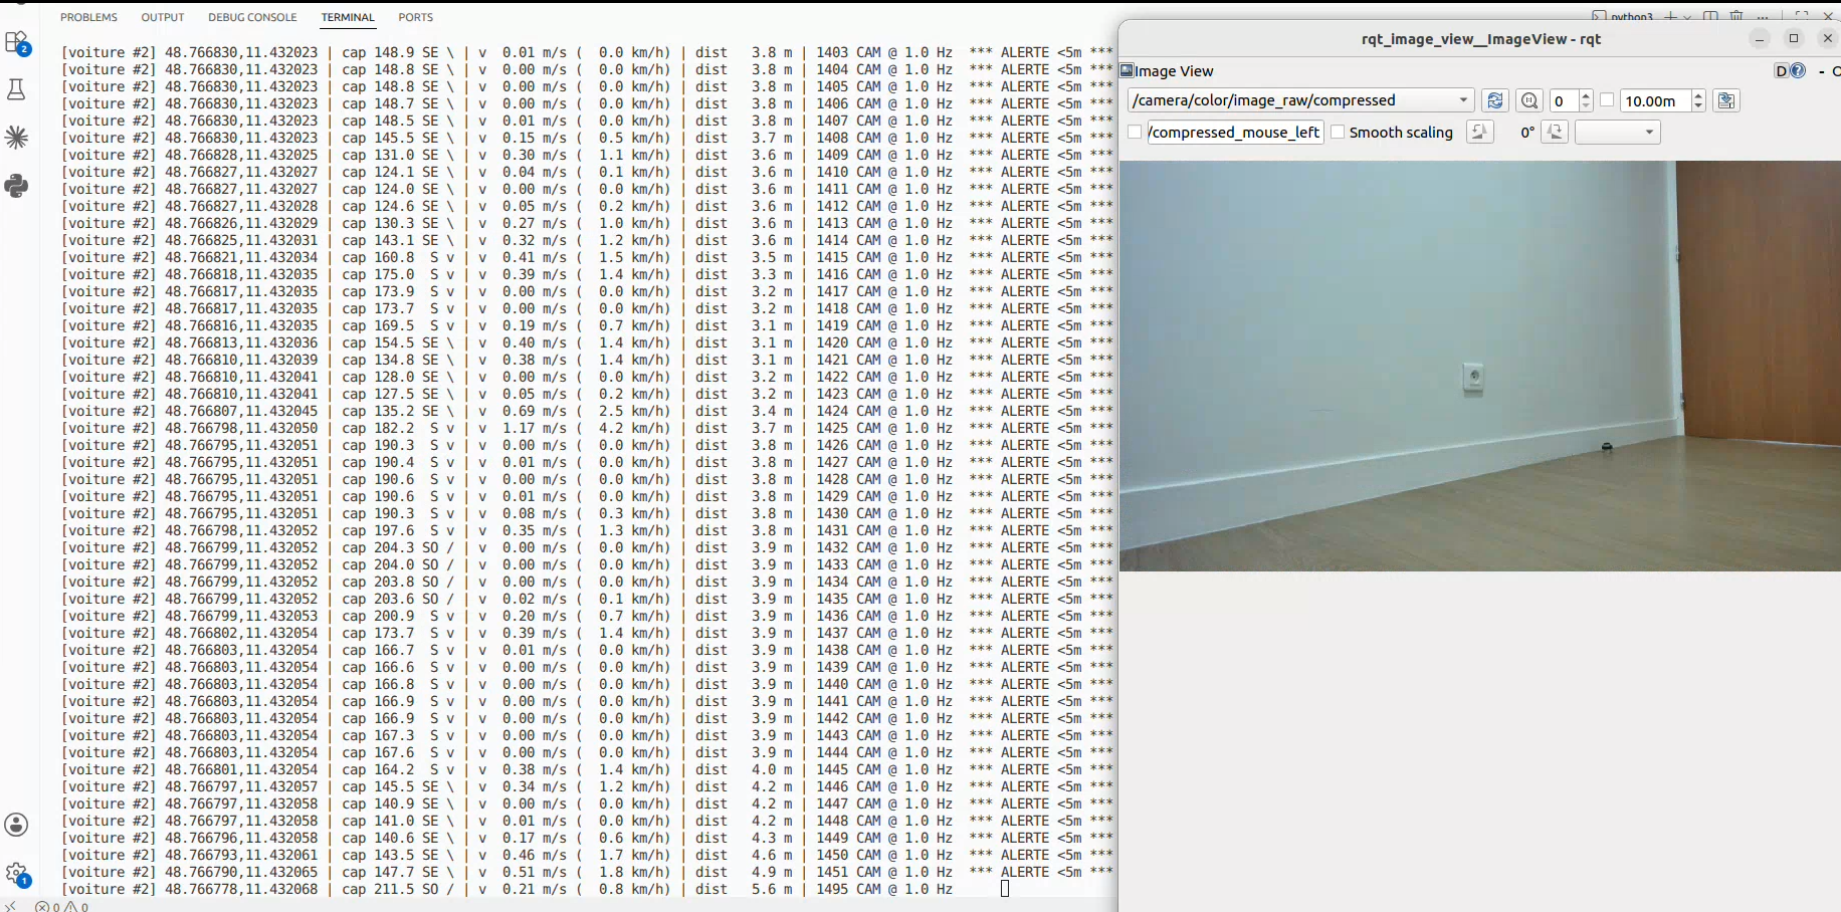
\includegraphics[width=0.9\textwidth]{img_cam_monitor.png}
\caption{Réception des CAM en direct : position, cap et vitesse du véhicule voisin.}
\end{figure}

\subsection{Perception intelligente --- YOLO + profondeur}
J'ai ajouté la \textbf{détection d'obstacles} par réseau de neurones \textbf{YOLO} sur la caméra,
avec estimation de la \textbf{distance} par la profondeur (en retenant le point le plus proche de
l'objet, plus fiable).

\begin{figure}[h]\centering
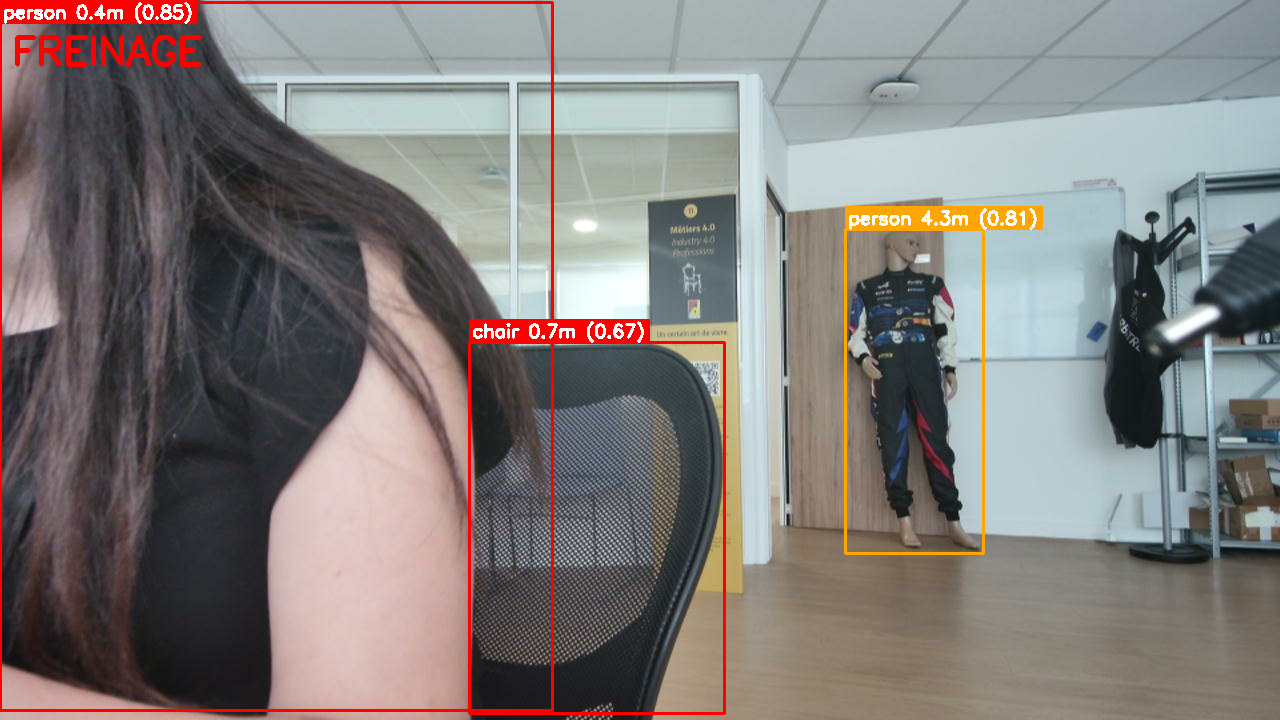
\includegraphics[width=0.66\textwidth]{img_detection_yolo.png}
\caption{Détection en temps réel : classe, distance et niveau de danger (rouge = obstacle proche).}
\end{figure}

\subsection{Alerte coopérative --- les messages DENM}
J'ai développé le message d'événement \textbf{DENM} (absent de l'outil de base) : quand un
obstacle est détecté, le véhicule \textbf{diffuse une alerte} normalisée que les autres véhicules
reçoivent et affichent.

\begin{figure}[h]\centering
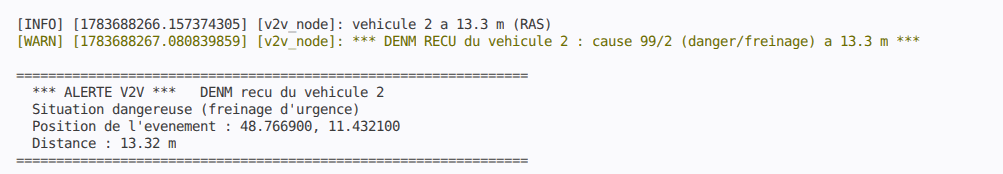
\includegraphics[width=0.8\textwidth]{denm_msg2.png}
\caption{Alerte reçue sur le véhicule voisin : cause, position et distance de l'événement.}
\end{figure}

\subsection{Freinage d'urgence automatique --- AEB}
Enfin, j'ai couplé la perception à l'actionneur : un \textbf{freinage d'urgence gradué} qui
exploite les trois sorties de YOLO --- la \textbf{distance} (freinage progressif), la
\textbf{classe} (priorité au piéton) et la \textbf{position} (uniquement les obstacles dans la
trajectoire) --- tout en préservant la direction du conducteur.

\begin{win}\textbf{Résultat :} une boucle de sécurité coopérative complète ---
\emph{percevoir $\to$ alerter $\to$ freiner}.\end{win}

% ================= ARCHI =================
\section{L'architecture finale}
\begin{figure}[h]\centering
\resizebox{0.96\textwidth}{!}{%
\begin{tikzpicture}[font=\footnotesize,
  b/.style={draw, rounded corners=2pt, align=center, minimum height=8mm, inner sep=3pt, fill=white},
  fl/.style={-{Latex[length=2mm]}, thick}]
  \node[b, fill=safe!12, draw=safe] (cam) {Caméra};
  \node[b, fill=safe!12, draw=safe, right=5mm of cam] (yolo) {YOLO + profondeur\\ \scriptsize détection + distance};
  \node[b, fill=safe!12, draw=safe, right=5mm of yolo] (dec) {Décision\\ \scriptsize danger ?};
  \node[b, fill=safe!20, draw=safe, below=5mm of dec] (aeb) {\textbf{AEB}\\ \scriptsize freinage gradué};
  \node[b, fill=auto!12, draw=auto, right=6mm of dec] (denm) {\textbf{DENM}\\ \scriptsize alerte V2V};
  \node[b, fill=auto!12, draw=auto, right=6mm of denm] (other) {Autre véhicule\\ \scriptsize \textbf{ALERTE}};
  \node[b, fill=teleop!12, draw=teleop, below=5mm of aeb] (car) {Voiture\\ \scriptsize direction + moteur};
  \draw[fl, safe] (cam)--(yolo); \draw[fl, safe] (yolo)--(dec);
  \draw[fl, safe] (dec)--(aeb); \draw[fl, teleop] (aeb)--(car);
  \draw[fl, auto] (dec)--(denm); \draw[fl, auto] (denm)--(other) node[midway, above]{\scriptsize WiFi};
  \node[b, fill=auto!12, draw=auto, left=6mm of cam] (cams) {CAM\\ \scriptsize position/cap/vitesse};
  \draw[fl, auto, dashed] (cams)--(cam.west);
\end{tikzpicture}}
\caption{Le véhicule perçoit (YOLO), décide, \textbf{freine} (AEB) et \textbf{alerte} les autres
(DENM), tout en partageant sa présence (CAM).}
\end{figure}

% ================= BILAN =================
\section{Bilan et perspectives}
\begin{note}[Ce qui fonctionne aujourd'hui]
Téléopération 5G supervisée $\bullet$ autonomie (SLAM/Nav2) $\bullet$ communication V2V (CAM
enrichis, échange bidirectionnel) $\bullet$ détection d'obstacles par IA avec distance $\bullet$
alerte coopérative DENM (boucle validée entre deux véhicules) $\bullet$ freinage d'urgence gradué.
\end{note}

\textbf{Prochaines étapes :}
\begin{enumerate}[leftmargin=1.5em, itemsep=1pt]
  \item \textbf{embarquer la perception} (YOLO) sur la Jetson pour une réaction autonome à bord ;
  \item \textbf{fusionner LiDAR + caméra} (géométrie + sémantique) pour une détection plus sûre ;
  \item essai du \textbf{freinage physique} sur la voiture, puis réglage des seuils ;
  \item \textbf{démonstration sur 5G} et \textbf{messages signés} (sécurité C-ITS complète).
\end{enumerate}

\vspace{4pt}\hrule
{\footnotesize\itshape Normes : ETSI EN 302 637-2 (CAM), EN 302 637-3 (DENM) ; pile Vanetza.
Documents détaillés : \code{rapport\_hebdo\_v2v\_denm.tex}, \code{recap\_v2v\_cam\_denm.tex}.}

\end{document}
